\documentclass[a4paper]{elsarticle}
\usepackage[utf8]{vietnam}
\usepackage{amssymb, amsthm, amsmath}
\usepackage{lipsum}	
\usepackage[locale=DE]{siunitx}
\usepackage[version=3]{mhchem}
\usepackage{graphicx}
\usepackage{setspace}
\usepackage{float}
\usepackage{caption}
\usepackage{capt-of}
\usepackage{subcaption}
\usepackage{mathtools, cuted}
\usepackage{titletoc}
\usepackage{anyfontsize}
\usepackage{sectsty}
\usepackage{makecell}
\usepackage{cases}
\usepackage{bm}
\sectionfont{\fontsize{13}{15.6}\selectfont}
\usepackage{caption}
\usepackage{indentfirst}
\DeclareCaptionFont{xipt}{\fontsize{13}{15.6}\selectfont}
\usepackage[font=xipt,labelfont=bf]{caption}
\usepackage[left=3.5cm,right=2.0cm,top=3.5cm,bottom=3.0cm]{geometry}
\usepackage{times}
\biboptions{numbers,sort&compress}
\usepackage[breaklinks,colorlinks=true,citecolor={black}, linkcolor= {black}, urlcolor ={black}]{hyperref}

% ====================================================================================
\begin{document}
\onehalfspacing
\fontsize{12}{15.6}\selectfont
\begin{titlepage}
		\begin{center}
\textbf{ĐẠI HỌC QUỐC GIA THÀNH PHỐ HỒ CHÍ MINH}\\
\textbf{TRƯỜNG ĐẠI HỌC KHOA HỌC TỰ NHIÊN}\\
	\noindent\rule{4cm}{0.4pt}
\end{center}
\vspace{10pt}
\fontsize{13}{15.6}\selectfont
\begin{center}
	\textbf{LƯƠNG HOÀNG SANG}\\
	Mã số học viên: 22C31009
\end{center}
\fontsize{16pt}{15.6pt}\selectfont
\vspace{20pt}
\begin{center}
	\textbf{ĐỀ CƯƠNG NGHIÊN CỨU ĐỀ TÀI\\ LUẬN VĂN THẠC SĨ
	}
\end{center}

\vspace{20pt}
\fontsize{12}{15.6}\selectfont
\begin{tabular}{p{3cm}p{11cm}}
	Tên đề tài: & \textbf{Khảo sát sự phụ thuộc của lực áp suất bức xạ lên lớp graphene bên trong một vi hốc cộng hưởng theo hướng tới của chùm sáng kích thích}\\
	&\\
	Ngành: & \textbf{Vật lý lý thuyết và vật lý toán}\\
	Mã số ngành: &\textbf{8440103}
\end{tabular}
\vspace{2cm}\\
\begin{minipage}{0.5\textwidth}
\begin{center}
	\textbf{Xác nhận của hướng dẫn chính}\\
	\textit{(Ký tên và ghi rõ họ tên)}\\
	\vspace{2.5cm}
	TS. Nguyễn Duy Vỹ
\end{center}
\end{minipage}
\hfill
\begin{minipage}{0.5\textwidth}
	\begin{center}
		\textbf{Xác nhận của đồng hướng dẫn}\\
		\textit{(Ký tên và ghi rõ họ tên)}\\
		\vspace{2.5cm}
		TS. Nguyễn Hữu Nhã
	\end{center}
\end{minipage}


\vspace{1cm}

\begin{center}
	\textbf{Thành phố Hồ Chí Minh, tháng 6 năm 2024}
\end{center}
\end{titlepage}
\newpage
\fontsize{13}{15.6}\selectfont
\section{Giới thiệu tổng quan} 

Hiện nay, vật liệu 2D đang có tiềm năng ứng dụng lớn trong các lĩnh vực như y học, quang điện tử, cảm biến \cite{H.Zhang, P.G.Steeneken}. Bên cạnh đó, sự phát triển của kĩ thuật chế tạo vật liệu tiên tiến đã hỗ trợ cho việc bóc tách vật liệu đơn lớp hoặc hai lớp phục vụ nghiên cứu các hiệu ứng quang - cơ. Việc tăng lực quang học tác dụng lên các lớp vật liệu cỡ micro và nano là rất quan trọng để điều khiển về mặt động lực học nhằm nghiên cứu các hiệu ứng ở ranh giới cổ điển và lượng tử. Chủ đề này cũng đã thu hút được nhiều sự quan tâm từ các nhà nghiên cứu. Chẳng hạn, nhóm của Zhang và các cộng sự \cite{Zhang2015} đã chứng minh rằng graphene có thể được đẩy bởi lực cảm ứng ánh sáng. Gần đây, Miller và các cộng sự \cite{Miller} đã đo chuyển động và lực trên tấm graphene được treo như một dao động tử điều hoà cơ học để thu được sự phân bố không gian của lực quang học theo kích thước của điểm laser hội tụ.  

Trong bài báo \cite{ThayVy} chúng tôi đã khảo sát về mặt lý thuyết khả năng tăng cường lực áp suất bức xạ (Radiation presure force, viết tắt là lực RP) lên lớp graphene đặt trong vi hốc cộng hưởng Fabry – Perot. Vi hốc được tạo bởi hai lớp vàng có bề dày mỗi lớp lần lượt là $t_1=\SI{47}{\nano\meter}$ và $t_2=\SI{80}{\nano\meter}$. Hai lớp vàng được đặt cách nhau khoảng $L_{OMC}=\lambda-\left(t_1+t_2\right)\approx\SI{565}{\nano\meter}$, với $\lambda$ là bước sóng laser $\ce{He}-\ce{Ne}$ chiếu vào vi hốc. 
\begin{figure}[h]
	\centering
	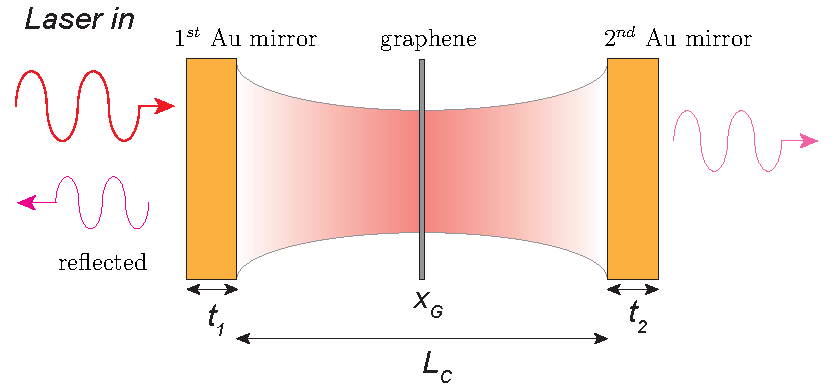
\includegraphics[width=0.8\linewidth]{figs/Hinh1}
	\caption{Mô hình vi hốc cộng hưởng (OMC) tạo bởi hai lớp vàng, lớp graphene được đặt ở giữa vi hốc.}
	\label{fig:1}
\end{figure}\\
Kết quả tính toán cho thấy rằng, lực RP tác dụng lên lớp graphene có thể đạt tới $\SI{36}{\pico\newton/\milli\watt}$ nếu graphene được đặt ở tâm vi hốc. Đặc biệt, độ cứng quang học của lớp graphene trong vi hốc có thể đạt tới $\sim\SI{30}{\pico\newton}/\lambda$, cho phép điều khiển và làm mát graphene chỉ bằng việc sử dụng lực RP.
\section{Mục đích nghiên cứu}
Chúng tôi mong muốn kiểm tra về mặt lý thuyết ảnh hưởng của hướng chùm sáng đến lực RP tác dụng lên lớp graphene trong vi hốc cộng hưởng. 
\section{Đối tượng nghiên cứu}
Sự phụ thuộc của lực RP tác dụng lên lớp graphene bên trong vi hốc cộng hưởng theo hướng tới của chùm sáng kích thích.
\section{Phương pháp nghiên cứu}
\begin{itemize}
	\item Tensor ứng xuất Maxwell (Maxwell’s stress tensor).
	\item Phương pháp ma trận truyền (Transfer matrix method) được đề xuất bởi \cite{ZhanTMM}.
\end{itemize}
Với phương pháp, các thành phần điện trường và từ trường sẽ được tìm từ hệ phương trình điều kiện biên tại mặt tiếp giáp giữa hai lớp:
	\begin{subnumcases}{}
		\textbf{n}\times\left(\textbf{E}_2-\textbf{E}_1\right)=\textbf{0}\\
		\textbf{n} \times\left(\textbf{H}_2-\textbf{H}_1\right)=\textbf{J}
	\end{subnumcases}
Trong đó, $\left(\textbf{E}_1, \textbf{H}_1\right)$ và $\left(\textbf{E}_2, \textbf{H}_2\right)$ lần lượt là thành phần điện trường và từ trường ở hai bên mặt phân cách, $\textbf{n}$ là vector pháp tuyến của mặt phân cách giữa hai môi trường, $\textbf{J}=\sigma \textbf{E}$ là vector mật độ dòng.\\
Sau khi tìm được các thành phần điện trường tới $E_i$ và điện trường khúc xạ $E_r$ qua mỗi lớp để thay vào tensor ứng xuất Maxwell $\textbf{T}$ thì lực RP tác dụng lên mỗi lớp được tính
\begin{equation}
	F_\text{RP}=\left\langle\int_{S}\textbf{T}\left(\textbf{r}, t\right)\cdot\textbf{n}\left(\textbf{r}\right)dS\right\rangle
\end{equation}
với  $\left\langle\dots\right\rangle$ là trị trung bình theo thời gian.

\section{Nội dung và phạm vi của vấn đề sẽ đi sâu nghiên cứu}
\begin{itemize}
	\item Tìm hiểu tính chất quang học của graphene, tensor ứng xuất Maxwell, phương pháp ma trận truyền cho bài toán quang học, lực áp suất bức xạ trên màng mỏng, \dots
	\item Sử dụng ngôn ngữ lập trình Python trong việc tính toán thành phần điện trường qua các lớp.
	\item Khảo sát sự phụ thuộc của lực RP tác dụng lên lớp graphene bên trong vi hốc cộng hưởng theo hướng tới của ánh sáng kích thích.
\end{itemize}
\section{Nơi thực hiện đề tài nghiên cứu luận văn}
Trường Đại học Khoa học Tự nhiên - Đại học Quốc gia Tp.HCM.
\section{Thời gian thực hiện}
Từ tháng 5/2024 đến tháng 11/2024:
\begin{center}
	\begin{tabular}{|>{\centering\arraybackslash}m{5cm}|>{\centering\arraybackslash}m{10cm}|}
		\hline
		\textbf{Thời gian} & \textbf{Nội dung}\\
		\hline
		\makecell{05/2024 - 06/2024} & Nghiên cứu cơ sở lý thuyết của đề tài, tìm hiểu các công cụ hỗ trợ: Python.\\
		\hline
		06/2024 - 11/2024 & Thực hiện đề tài luận văn.\\
		\hline
		11/2024 -  12/2024 & Chỉnh sửa nội dung báo cáo, chuẩn bị bảo vệ luận văn tốt nghiệp.\\
		\hline
		Tháng 12/2024 & Bảo vệ luận văn tốt nghiệp.\\
		\hline
	\end{tabular}
\end{center}
\bibliographystyle{elsarticle-num}
\bibliography{SangRef_2024}
\end{document}


